\documentclass[a4paper,11pt]{memoir}

\usepackage[utf8]{inputenc}
\usepackage[T1]{fontenc}
\usepackage[danish,english]{babel}
\usepackage[urw-garamond]{mathdesign}
\usepackage{minted}
\usepackage{graphicx}
\usepackage[status=draft]{fixme}
\usepackage{amsthm}
\usepackage{xcolor}
\usepackage{amsmath}
\usepackage{wallpaper}
%\usepackage{changepage}
\usepackage[margin=10pt,font=small,labelfont=bf,labelsep=endash]{caption}

\usepackage[
  backend=biber,
  backref=true,
  style=numeric,
  sorting=none,
  citestyle=numeric]{biblatex}
\addbibresource{citations.bib}

\definecolor{mycolor1}{HTML}{00507E}
\usepackage[
  pdfauthor={Truls Asheim},
  pdftitle={Implementing High Peformance Synchronous Message Exchange},
  colorlinks=true,
  linkcolor=mycolor1,
  citecolor=mycolor1,
  urlcolor=mycolor1,
  filecolor=mycolor1]{hyperref}
\usepackage[noabbrev,nameinlink]{cleveref}

% Convert our figures
\immediate\write18{make svgfigures}

% Set up captions
%\captionnamefont{\small\bfseries}
%\captiontitlefont{\small}
%\captionwidth{0.8\linewidth}

% enumerate subsections
\setsecnumdepth{subsection}

\fxsetup{margin}

\theoremstyle{definition}
\newtheorem{property}{Property}

%\title{Implementing high performance Synchronous Message Exchange\\
%       University of Copenhagen}
%\author{Truls Asheim \texttt{<truls@asheim.dk>}}
%\date{}

\begin{document}
\begin{titlingpage}
\thispagestyle{empty}
\ULCornerWallPaper{1}{img/nat-farve.pdf}
\ULCornerWallPaper{1}{img/diku-en.pdf}
\begin{adjustwidth}{-1.75cm}{-1.5cm}
\vspace*{-1cm}
\textbf{\huge Bachelor's Thesis} \\
\vspace*{2.5cm} \\
\textbf{\Huge Implementing High Performance Synchronous Message Exchange} \\
%\vspace*{.1cm} \\
%{\huge An Eventual Consistent Parallel Block Device} \\
\begin{tabbing}
  Truls Asheim ~~ \= \texttt{<truls@asheim.dk>} \\[14.3cm]
  \textbf{\Large Supervisor} \\
  Brian Vinter \> \texttt{<vinter@nbi.dk>}
\end{tabbing}
\end{adjustwidth}
    %\newpage
    \ClearWallPaper

\end{titlingpage}
%\begin{titlingpage}
%\maketitle
%\end{titlingpage}


\begin{abstract}
  Synchronous Message Exchange (SME) is a messaging framework similar
  to Concurrent Sequential Processes (CSP) aimed at modeling
  synchronous systems such as hardware. With the goal of faster
  execution of SME networks, various models for parallelized execution
  of SME networks have been designed, implemented and benchmarked.

  We give an overview of the properties of SME and explain how they act in a
  parallelized environment. We then explain the details of our
  implementation and finally measure our implementation through
  various benchmarks. We have found that the achievable speedups are
  highly dependent on the kind of work performed by a
  network. However, one of our the models that we have implemented
  proved extremely successful and is capable of achieving near linear
  speedups.
\end{abstract}

\begin{otherlanguage}{danish}
\begin{abstract}
  Synchronous Message Exchange (SME) er et Concurrent Sequential
  Processes (CSP) lignende messaging framework som er rettet imod
  modellering af synkrone systemer så som hardware. Med en målsætning
  om at muliggøre hurtigere eksekveringer af SME netværk, har vi
  designet, testet og implementeret forskellige modeller for
  parallelisering af SME modellen.

  Vi vil give et overbliv over egenskaber ved SME modellen og hvordan
  de fungerer i et paralleliseret miljø. Vi vil derefter forklare
  detaljer ved vores implementering og endeligt vil vi undersøge
  ydelsen af vores implementering igennem forskellige målinger. Vores
  konklusion er at den mulige hastighedsforbedring i høj grad afhænger
  af hvilken type arbejde som bliver udført af de netværk vi
  kører. Dog har en af vores modeller vist sig yderst succesfuld og
  skalerer linært i forhold til antallet af processorer.
\end{abstract}
\end{otherlanguage}

\clearpage
\tableofcontents\clearpage
\listoffigures

\chapter{Introduction}

\section{Project description}
In this report, we describe the design and implementation of a highly
efficient library for parallel execution of new, globally synchronous,
message passing framework called Synchronous Message Exchange
(SME). We will

In this report, we describe a synchronous message passing framework
intended to aid simulation of applications whose operating semantics
are compatible with the SME model

\section{Hardware Description Languages}
A Hardware Description Language (HDL) is a programming language for
describing hardware designs. A program written in such a language is
usually

\section{Background and Motivation}
Field-programmable Gate Arrays (FPGA) provides several advantages over
using GPGPUS for processing work including a significantly improved
performance-per-watt ratio. Due to the low-level nature of current
tools for programming FPGAs, their use are largely restricted to
engineers with working knowledge in the field of hardware design. In
order for software developers to take advantage of FPGAs, improved
high-level hardware design utilities are required \cite{bacon2013fpga}.

The creation of SME was motivated by attempts to use CSP for modeling
hardware which, for simple cases, proved successful
\cite{rehr2013bpu}, but additional testing revealed that the CSP model
introduced a significant overhead when simulating more complicated
hardware designs. Modeling the clock-cycle driven global synchrony
that exists in hardware proved to be particularly difficult with CSP
and required the introduction of several additional processes and
channels. This added complexity reduced simulation performance and
limited the usefulness of the CSP-based hardware design model \cite{vinter2014synchronous}.

SME is an attempt to provide a programming framework that, while
leveraging and maintaining the properties of CSP that proved useful
and f enforcing a hardware-like paradigm, that is accessible to
software developers. By \cite{vinter2014synchronous}

\section{Limitations}
This report will not discuss details related to design of hardware

\section{Related work}
Discuss master thesis

%%% Local Variables:
%%% mode: latex
%%% TeX-master: "master"
%%% TeX-command-extra-options: "-enable-write18"
%%% End:

\chapter{Analysis and Design}
In this chapter, we will describe and justify the design of our library and the
thought and considerations that went into producing the final design
and ideas that was discarded along the way.

\section{Overall goal and success parameters}



% \section{Programming}
% Even though the eventual goal of the SME-library is to enable
% generated networks to execute
% The API exposed to the user of the SME library should be designed with
% a focus on balancing expressiveness and ability to be easily
% understandable....

% The API implemented by \cite{vinter2014synchronous} is heavily
% dependent of the highly dynamic nature of the Python programming
% language used to implement their prototype. Since our implementation
% is written in C++ we cannot directly mimic the python API in our
% implementation. Given the similarities between SME and CSP it seems
% obvious to let us inspire by

\section{Paralellization model}

A common way of parallelizing CSP-like networks is to use user-level
threads to represent a process. In comparison with OS-level threads,
user-level threads has a significantly lower overhead both with
regards to context switching penalty and memory cost. Due to these
limitations, implementing these kinds of message passing systems using
only OS-level threads are generally not feasible. Therefore,
user-level threads are used by other message passing systems such as
the C++CSP library\cite{brown2003introduction} and the goroutines in
the Go language\cite{deshpandeanalysis}. However, implementing a
user-level threading library would add complexity to our
program since we would need to implement a scheduler, for scheduling
processes on top of OS-level threads.

Comparing, once again, to CSP, the concurrency in CSP is inherently
asynchronous while SME is entirely synchronous in nature. This means
that a CSP library needs to implement a scheduler which decides when
to give control to a process based on certain events, e.g. a process
wishing to communicate or a process receiving a message from another
process. \fxnote{Repeats some of previous paragraph}.

Our original design considerations centered around such a design,
however, due to the enforced synchrony of SME we don't have the same
need to schedule processes ``intelligently''. We know that all
processes needs to run during a cycle and all busses have to propagate
their values. This, in addition to he shared nothing property of SME,
allows us to specify a much simpler parallelization model for SME
compared to the techniques used by the aforementioned message passing
network implementations:

The basic idea that we base our design on is conceptually similar to a
classic producer-consumer setup. In our case, the work ``produced'' is
the processes to be executed, and the consumers are the threads
executing the processes. In this setup, a process is run simply by
calling a function, whereas user-level threads are usually implemented
using the \texttt{setcontext} and \texttt{getcontext} library
functions, which, while extremely fast, still causes a slightly larger
overhead compared to a simple function call. \fxnote{Switching between
  OS-level processes is actually really fast, since context-switching
  from one process to another usually only involves moving CPU
  registers, i.e. the stack pointer, to an appropriate location, TODO
  write something like that}

by simply letting a number of OS-threads run SME processes in a
worker-consumer like manner. This approach also make it simple enforce
the synchronicity properties of SME, since we know hen a process has
finished executing. Unlike

In this project, we have explored two different variations of this
basic idea. Both models are based on the idea described in the
previous paragraph. Our overall goal in parallelizing execution of
SME-networks is to minimize the amount of core idle time. We expect
the hereafter presented model to achieve this goal under different
circumstances \fxnote{different networks}.



\subsection{Pros and cons}
Pros: Shared nothing,forced synchrony 

Cons: Forced syncrhony 

\subsection{``Worker quwue'' model}
This approach is similar to a classic producer-consumer model where we
have a number of workers which takes tasks off a circular queue and
executes the processes. The main advantage of this model is that it
allows processes with different execution times to ``interleave''
leading to a higher overall execution time. The primary problem of
this model is that we need to make the queue thread-safe. The locking
mechanism needed to do this isn't free, and could therefore come at a
significant cost when we're executing a network consisting of small
processes.

\subsection{Static orchestration model}
In this model, we assign separate queues to each thread of execution
and distribute the processes amongst them. Due to the properties of
SME, this distribution of processes only needs to happen once, before
we start network execution. The main advantage of this model is that
eliminates any shared state in our network, and therefore we don't
need to consider the thread-safety of our queues. This reduces the
fixed cost of executing a process significantly. This model, however,
is more sensitive to uneven distributions in process workloads. For
instance, if we end up assigning predominantly small processes to one
core and large processes to another, the core executing the small
processes would be left idle until the other core has finished
executing it's part of the cycle.


Overall, we expect the latter model to have a significant advantage in
executing networks with small processes while the queue-locking cost
of the former model will perform better when executing networks with
large or unevenly distributed workloads since the queue-locking costs
owill be amortized and allow its process-interleaving ability to shine
through.

%Using OS-level threads for representing the SME processes was quickly
%ruled out during the design process. OS-level threads are severely
%limited in that the number of threads a process can have is highly
%limited \fxnote{Find reference for number of threads per process} and
%switching between OS-level threads is very expensive compared to, for
%instance, user-level threads. \cite{sung2002comparative}\fxnote{Find
%  more recent citation for the performance of OS vs. user-level threads}.

%Using user-level threads, on linux implemented by using the (now
%deprecated) \texttt{setjump, longjump} functions or the more current
%\texttt{ setcontext, getcontext} functions, is another possible way of
%implementing our networks. The notion of a user-level thread is highly
%compatible with our concept of a process, namely
%\fxnote{finish}. User-level threads is the method that is used to
%implement many CSP libraries, including C++CSP2.

%One important difference between the CSP and SME execution models is
%that CSP is asynchronous and event-driven in nature while SME is, as
%previously mentioned, entirely synchronous. This allows us to take a
%significantly more simple approach to scheduling threads compared to
%C++CSP. A parallel CSP library needs to schedule a process for
%execution based on events generated by other processes
%\cite{brown2003introduction}. In SME we know that every process needs
%to run \fxnote{This needs to be better described} during every ``clock
%cycle''. This greatly simplifies our implementation of multi-threaded
%SME.

The optimal way of showing 

\subsection{Identifying optimal process scheduling}
In order to determine the efficiency of various methods of process
scheduling we need to identify the optimality condition for our
process scheduling. An illustration of our threading model can be seen in
\cref{fig:suboptdist}. The green boxes represents processes while the
red boxes indicates core idle time. Notice, how we by redistributing
the processes across threads could reduce the idle-time of our
cores.


\section{Synchronizing cycles}
The main problem of executing an SME network is to make sure that the
cycles are synchronized, or that all the processes ``meet up'' at the
end of an execution cycle. While the problem of executing the actual
processes, due to the shared-nothing property of SME, is embarrassingly
parallel, the need for synchronization makes it not quite
so. Therefore, the time spent on synchronization will significantly
impact the overall performance of our network.

\fxnote{Talk about barriers somewhere, which probably describes some
  of what we're talking about more accurately}

\begin{enumerate}
\item In order to know when to stop executing, we need to count the
  number of cycles performed
\item In order to know when a cycle is complete, we need to keep track
  of the number of processes that has been executed.
\end{enumerate}

\subsection{Cost of synchronization}
The cost of synchronization arises from two areas


There are two places in the network execution where this
``accounting'' could be preformed. We could either place a ``guard''
around each ... An alternative way of performing synchronization is to
insert special p

``Naive'' way of doing would be to let each execution thread count the
number of processes that has been executed. The problem with this
approach is that it adds a fixed computational cost to each process
execution. This would become especially pronounced in model 1
which would require 

Furthermore, we would need to keep the state of the network
as a global shared state which would need to be protected by locks
when accessed by a thread. Both of these factors would significantly
limit the concurrent scalability of the parallel execution. 

One of the central parts of managing an execution cycle is how we
synchronize our threads before leaving each cycle phase
\fxnote{elaborate}. In order to maintain the previously described
synchrony property, ... Furthermore, the network execution must be
controlled so that we are able to stop the execution after a specified
number of cycles has completed.


An alternative method, which allows the 

\section{Implementing the queues}
An actual circular linked list where the last element points to the
first would be the most natural representation of the conceptual
circular queue that we just described. The usual advantage of using a
linked-list structure is that it allows for O(1) addition of
elements. The disadvantage if that element access is slower, even
though we would never need to actually traverse the list in order to
find a specific element, the cost associated with simply getting the
next element of linked list is not insignificant when performed enough
times \fxnote{crap}

A straight-forward array is much better suited for the task z7

\subsection{Locking primitices}
Classic locking mechanisms such as semaphores and mutexes needs no
introduction. We will, however, spend a little bit of time on
explaining the new kid on the block -- atomic operations.  Atomic
operations 

\subsection{Process orchestration}
As we discussed in the previous section, the primary limiting factor
for our multi-threaded network is an uneven and suboptimal
distribution of processes across CPU-cores. If no attempt is made to
optimize process distribution, the order of process execution will
depend on the order of which processes are defined in the source
code. Due to \cref{noshare} and \cref{synchro} of SME
networks there is no scenario where it would be necessary or
beneficial for a programmer to exercise ultimate control over the
order of process execution. Therefore, maximizing CPU-core utilization
would be an unreasonable burden to put on the programmer, especially
since their optimization efforts would be specific to a certain number
of CPU-cores.

The optimal method and timing of process orchestration depends on the
dynamicity \fxnote{is predictability a better word?} of the work
performed by the network we are executing. A network where each
process performs a fixed amount of work per iteration will only need
to be orchestrated once, while a network where the workload of the
processes are variable will need to be continuously evaluated at
runtime in order to maintain our optimality condition. These various
methods will be discussed for the remainder of this section.


\begin{figure}
\centering
\includegraphics{figures/parallel}
\caption[Proposed SME parallelization model]{Example of suboptimal
  distribution of processes across processing threads. Green blocks
  represents processes while red blocks represents thread idle
  time. Threads are named $p_{i,j}$ where $i$ is the number of the
  thread the process has been assigned to and $f_i$ is the combined
  idle time for each thread. Threads are named $t_i$.}

\label{fig:suboptdist}

\end{figure}




%\fxnote{Discuss/investigate problem of
%  ``optimization-looping''. Imagine a network where the execution time
%  of each process is completely random. This would most likely trigger
%  a reorchestration after every iteration which may end up taking more
%  CPU-time than the actual process execution.}

\subsection{Round-robin orchestration}
\begin{figure}
\centering
\includegraphics{figures/roundrobin}

\caption[Round-robin orchestration]{Illustration of round-robin
  process orchestration. Progressive iterations are shown as
 
 increasing color intensity of arrows}

\label{fig:roundrobin}

\end{figure}


Processes will be executed on the first available core as seen in
\cref{fig:roundrobin}




%\section{Testing correctness/Ensuring correctness/SME compliance testing}}

% This should be somewhere else
%In order to check the correctness of our implementation of the
%SME-model we use a simple test network which can only be executed
%correctly if our implementation of SME is obedient to all of the
%required SME-propertoes. This test network will henceforth be referred
%to as the \textit{validator netowrk} or simply the \textit{validator}.

%Our test network consists of a validator process and $n$ plusone
%proccesses. A single bus carries an output value from the validator to
%all of the plusone processes...

%A number of error conditions that might occur during network execution
%include
%itemize...

%If executed correctly, the network will maintain the following
%invariant:

%We still need to make sure that our test network is adequately
%capable of detecting possible error conditions that may occur during
%execution. To do this, we use fuzzing. Fuzzing is a well known
%technique from security research in order to find vulnerabilities in
%software and works by, in a random and unpredictable manner, providing
%unexpected and invalid input to programs.

%In essence, the idea is to test the hypothesis(/statement) that if the
%validator is able to correctly detect a working network, it should
%also detect an incorrectly  working network.

%We adapt the fizzing approach to our use case by introducing a number
%of processes to our network which, in an unpredictable manner,
%simulates a number of failures

%\begin{enumerate}
%\item A process fails to increment it's input value for a single
%  iteration
%\item A process falls behind on a value increment
%\item A process skips returning a value for a single cycle
%\item A process repeatedly receives 0 from a channel
%\item A process simply stops 
%\end{enumerate}

%The observant reader may wonder how we're going to test for failures
%in the value propagation phase. Our proposition is that bus-related failures
%are fully covered by the above cases. For instance, several of the
%above cases are the direct equivalent of a failing (or delayed) bus propagation

%%% Local Variables:
%%% mode: latex
%%% TeX-master: "master"
%%% TeX-command-extra-options: "-enable-write18"
%%% End:

\chapter{Implementation}
%%% Local Variables:
%%% mode: latex
%%% TeX-master: "master"
%%% End:

%\chapter{Conculsions}
% We have revealed some of the properties of SME. More real-world usage is still needed in order to decide on the optimal way to implement the network. We have given some options and shown that it is possible to support multiple execution models in the same framework. 

%%% Local Variables:
%%% mode: latex
%%% TeX-master: "master"
%%% TeX-command-extra-options: "-enable-write18"
%%% End:

\chapter{Benchmarks and Discussion}

We will present a number of benchmarks designed to compare and
quantify the differences in performance of the parallelization models
that we have implemented.

Since the execution time is only dependent on the total amount of work
that a network performs and not how the processes in the network are
connected, all of our benchmarks will use a ring-shaped
(\cref{fig:benchnetwork}) network with the participating processes
performing varying amounts of work.

We conjecture that the scalability of our implementation will depend
strongly on the nature of the workload performed by the SME-networks
benchmarked. We will therefore benchmark both light and heavy

As our previously presented hypotheses states, we expect our
benchmarks to show that the effects of syncing becomes more pronounced
as we decrease the amount of work performed by our processes while it,
on the other hand, will become amortized as the amount of work
performed by each process increases.

\begin{figure}
\centering
\includegraphics{figures/ring}
\caption[SME network used for benchmarking]{Illustration showing the
  layout of the network used for benchmarking. The blue circles
  represents processes and the arrows represents busses}
\label{fig:benchnetwork}
\end{figure}


\section{Testing methodology}
All of the time measurements shown were performed inside the SME
framework itself using the C++11 \texttt{<chrono>} functions, and
measures only the actual execution time of the network. It therefore
does not include the constant time required to generate the
benchmarked networks. Two different hardware platforms has been used
for performing the benchmarks: One AMD and one Intel platform.

The Intel machine has the following specs
\begin{itemize}
\item CPU: 1x Intel Xeon E3-1245 V2 @ 3.40GHz, 4 cores (8 threads)
\item RAM: 32GB
\item OS: Linux
\end{itemize}

and the AMD machines used are part of the eScience cluster at NBI and
boasts the following specs:
\begin{itemize}
  \item CPU: 2x AMD Opteron 6272 @ 2.1GHz, 16 cores
  \item RAM: 128GB
\end{itemize}

Since the instruction set used by the two CPU's support incompatible
optimizations, code generated for one of the CPU's will not run
unmodified on the other. Therefore, code executed on the AMD CPU were
compiled with the GCC flags \texttt{-mtune=barcelona
  -march=barcelona}, while code executed on the Intel CPU were
compiled with \texttt{-march=native} on a Core i7 machine. GCC 4.9 was
used in both cases. Furthermore, due to incompatible versions of
\texttt{libstdc++} on the test machines, all benchmarks has been
performed using statically linked binaries.

All of the benchmarks has been executed 5 times and the graphs are
based on the averages of these. Error bars showing the minimum and
maximum deviation from the average has been added to all graphs,
however, in some cases the deviations between benchmark runs were too small
for the error bars to be visible.
We have tried to size the workloads such that the running times are
kept within reasonable bounds \fxnote{elaborate}
We calculate our speedup using the formula


\begin{equation*}
S = \frac{T_{\text{old}}}{T_{\text{new}}}
\end{equation*}

where $S$ is the achieved speedup, $T_{\text{old}}$ is the original
(pre-improvement) speed and $T_{\text{new}}$ is the new
(post-improvement) speed \cite{hennessy2012computer}.

As a final note, when we talk about the workload of a cycle we refer
to the combined work of all processes in the network, not the work
performed by an individual process. As such, we define the workload of
the network as a function of both the work performed by the individual
processes and the number of processes participating in the
network. The raw benchmark data can be found in \cref{chap:benchdata}.

\section{Synchronization dominated}
In this section, we present a benchmark where the performance is
predominantly determined by the efficiency of the synchronization
mechanisms.

We perform this benchmark by creating a ring which does nothing other
than passing an integer value from process to process. Sine each
process only takes a few clock cycles to execute, we expect that this
benchmark will expose the overhead caused by synchronization.

The following source code used in the execution unit of the process
\begin{listing}
\begin{minted}{C++}
void step() {
  int val = in->read();
  out->write(++val);
}
\end{minted}

\caption{Source code for the execution unit of the processes
  participating in the network used for sync-dominated benchmarking}
\end{listing}

\begin{figure}
\centering
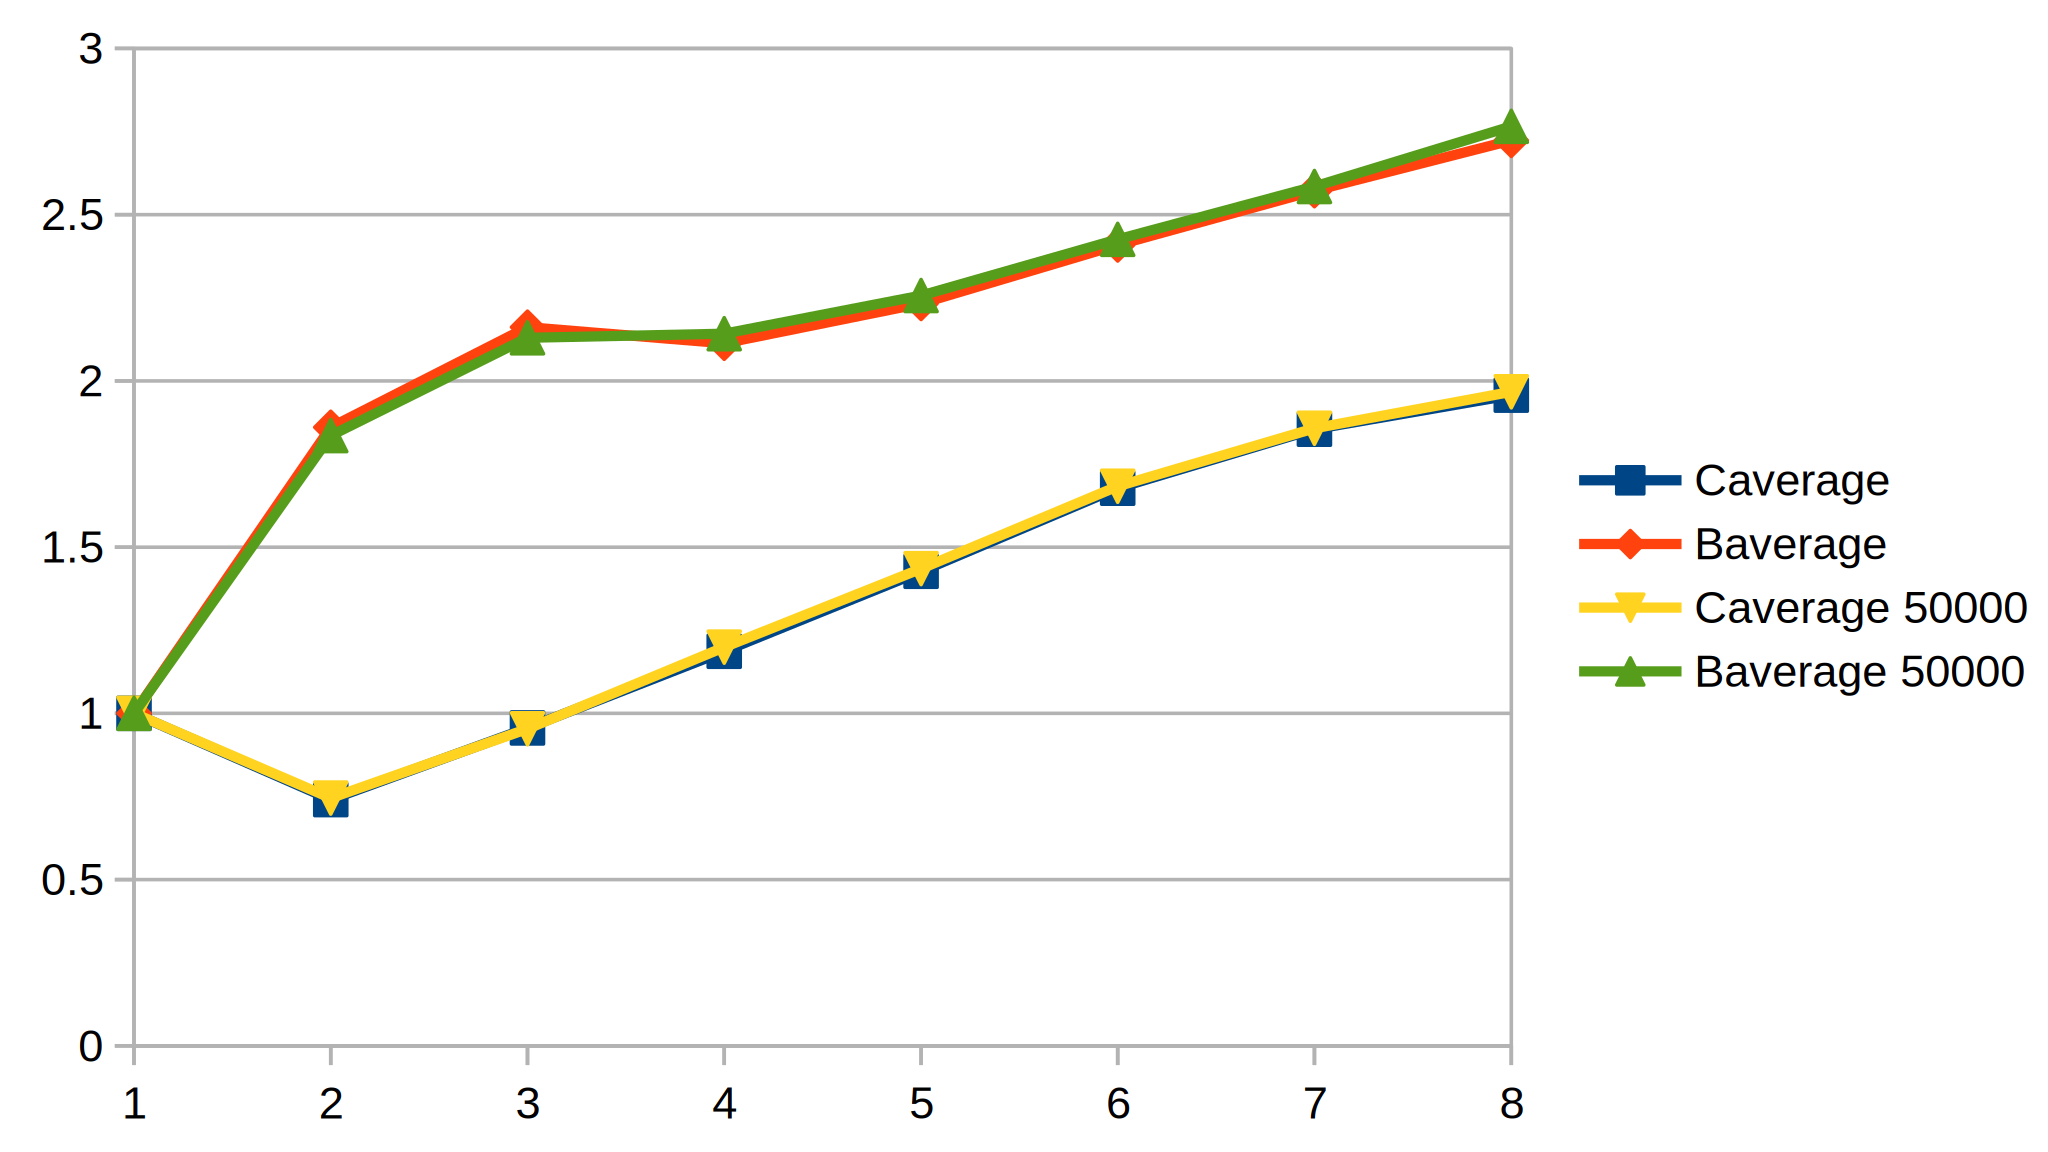
\includegraphics[width=\textwidth]{graphs/graphone}
\caption[Benchmark graph]{Graph showing the speedup of a SME network
  consisting of 20000 and 50000 processes respectively when executed
  for 50000 cycles on an Intel Xeon CPU}
\label{fig:intel-sync}
\end{figure}

\begin{figure}
\centering
\includegraphics[width=\textwidth]{graphs/amd-sync-20000}
\caption[Synchronization-dominated benchmark on AMD cluster]{Benchmark results for a network of 20000 processes running
for 100000 iterations on the AMD cluster}
\label{fig:amd-sync}
\end{figure}


\subsection{Discussion}
We can observe a number of things from the results that can bee seen
in \cref{fig:intel-sync}.  This benchmarks shows the performance of
two different networks, one with 20000 processes and one with 50000
processes. Both networks executed 100000 cycles.

When looking at the benchmark of the worker list model, one thing that
is clearly visible from this benchmark is the overhead produced by the
atomic increment that is required.. This model is doubly penalized
when running the benchmark since we, addition to then time required by
the atomic increment, which is performed before every process
execution, also need to wait for all of the threads to sync
up at the end of a cycle. What is slightly surprising, however, is the
actual performance that this method shows. It performs significantly
worse when going from one to two threads. The most likely explanation
for this result is CPU optimizations which make atomic updates of a
variable less costly when these updates only occures from one thread.

Our static orchestration model performs quite decently and produces
almost 2x speedup when going from 1 to 2 threads. When adding
additional threads, the speedup decreases, which is expected since the
time spent synchronizing is increased,

%\fxnote{which manifests as
%  dropping CPU-utilization. When running 4 threads, the CPU
%  utilization drops to 360\%, unfortunately, I probably wont have time
%  to measure or show this}

Common for both of the models, is that the size of the network
executed seems to have no impact on the relative speedups achieved.

Since the Xeon CPU that the benchmarks were performed on only have 4
cores with Hyper Threading, another interesting observation is that
Hyper Threading seems to give a significant additional speedup. One
hypothesis for explaining the cause of this is that branch-prediction
isn't very effective at predicting which functions we're going to call
in our SME network. A branch mis-prediction causes the CPU-pipeline to
be cleared, creating an optimal condition for Hyper Threading to make
use of the empty pipeline-stages\cite{fog2014microarchitecture} While
branch-predictors This hypothesis could be tested by running the
program through a profiler in order to measure the number of
mis-predictions occurring. At this time, these results are not
available.

\Cref{fig:amd-sync} show the results of the smallest version of the
benchmark running on the AMD cluster. The results are significantly
worse compared to the results of the Intel Xeon CPU, both in absolute
running times \fxnote{Is it OK to show the numbers?} and
speedup. Early possible explanations was that, due to the extremely
long running time of the benchmark, we were seeing the effects of the
process being moved between CPU-cores. However, the results remained
unchanged after pinning the threads to CPU-cores placed on the same
NUMA-unit. Thus, the only reasonable explanation explanation is that our
syncronization mechanisms is significantly less optimized on the AMD
CPU compared to the Intel CPU.

Another thing standing out from this benchmark is the huge variability
between the different benchmark runs as shown by the Y-axis error bars.

Due to these very poor initial benchmark results, we didn't attempt
benchmark the synchronization dominated network with different problem
sizes on the AMD-cpu.


\section{Cycle dominated}

\begin{figure}
\centering
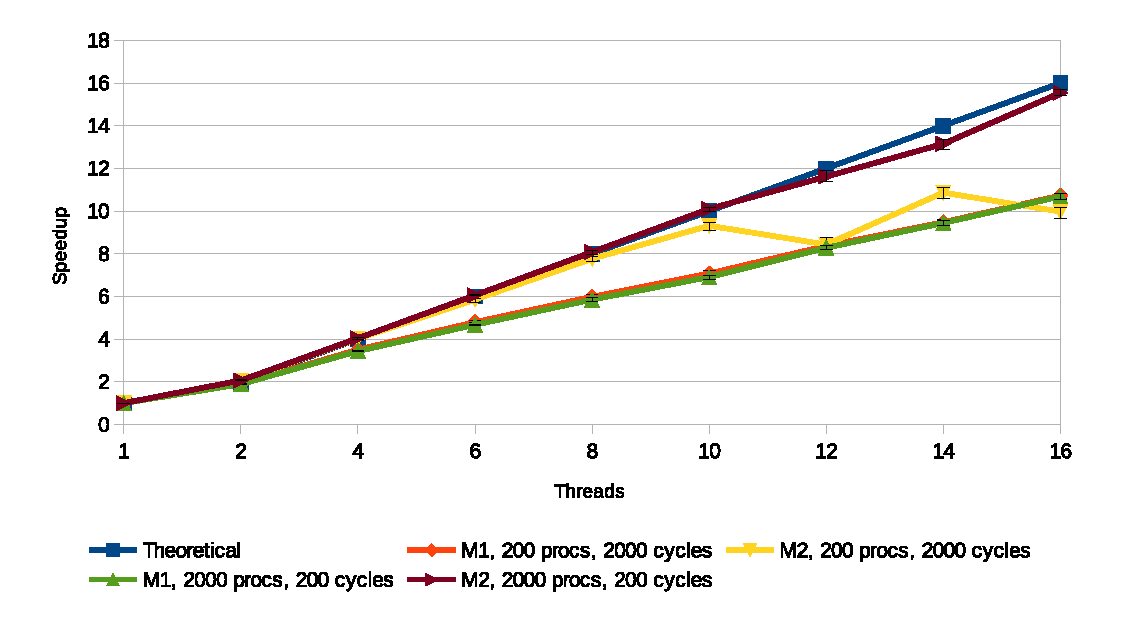
\includegraphics[width=\textwidth]{graphs/heavy-ring2}
\caption[Synchronization-dominated benchmark on AMD cluster]{Benchmark results for a network of 20000 processes running
for 100000 iterations on the AMD cluster}
\label{fig:heavy-ring}
\end{figure}


In this benchmark, the processes in the network performs a significant
amount work. We expect that this will, to some extent, amortize the
synchronization overhead inherent in the SME model. Combined with the
fact that the individual processes contain no shared state, we
conjecture that this benchmark will scale significantly better
than the previous synchronization dominated benchmark that we
performed.

The unit of work being performed by every process in every cycle is
simply to divide a \texttt{double} floating point number by 3, 10000
times. Since the busses in our SME-implementation only supports
transporting integer values nothing is being done with the value calculated,
but as long as our workload isn't being optimized away at compilation
time this is irrelevant.

The size of the workload and the number of nodes were chosen such that
the running times of the benchmarks would be reasonable \fxnote{elaborate}

We use floating point numbers as values as opposed to integer values
simply because they are more demanding of the CPU.
%\fxnote{Yes... good question, Why exactly do we do that?}

The following code is used as workload in our processes

\begin{listing}[H]
\begin{minted}{C++}
private:
  double n;
  int i;
protected:
void step() {
  n = 533.63556434;
  for (i = 0; i < 10000; i++) {
    n = n/3;
  }
  int val = in->read();
   out->write(++val);
}
\end{minted}
\caption{Code used for generating work in the cycle-dominated
  benchmarks}
\label{lst:cyclecode}
\end{listing}


\subsection{Discussion}
The overall conclusion that we can draw from this benchmark it that,
for workloads that are sufficiently large, the static orchestration
model exhibits significantly better speedups than then the work list
model.

The work list model, however, appears to be less sensitive to
variations in problem sizes since it performs produces similar
speedups in the two benchmarks that we have performed. It is
interesting that the overhead related to incriminating the atomic
pointer still has a noticeable negative impact on its performance. The
increased stability of the results can probably be attributed to the
continuous synchronization required by the work list which causes
neither of the threads falls behind or speeds ahead of the other
threads. Therefore, the combined time that the threads spends in the
synchronization barrier is smaller compared to the statically
orchestrated model.



Another thing that stands out in the graph is the curious zig-zag
pattern that that the statically orchestrated model in the benchmark
with the least amount of work forms when running across more than 10
threads. We assume this to be caused by the uneven distribution of
processes performed by the method described in the implementation
chapter, in the case of 200 processes distributed across 12 threads,
would assign 8 additional processes to one thread compared to the
others.

%ay something about NUMA units 

%The current algorithm for partitioning the processes into per
%thread work lists does a very bad job at maintaining an equal
%distribution when the number of processes does

%\fxnote{Not done, points I would like to mention}
%\begin{itemize}
%\item Adjusting the ratio of work-to-cycle impacts the speedup that we
%  can achieve when using the static orchestration model (as expected)
%\item I have no idea what causes the zig-zag patterns. They are due to
%  imbalances in process distribution.
%\item The worker-queue model (Model 1) produces identical results
%  independent of work-to-cycle. Probably because the single shared
%  queue used by all threads makes the threads meet up at the same time 
%\item The static-orchestration seems to, for sufficiently large
%  workloads, scale liberality, (Yay!)
%\end{itemize}

A problem with this benchmark is that the work that we perform can be
performed entirely within the cache of a CPU-core. This allows us to
scale more strongly than when benchmarking a problem which to a larger
extent is limited by memory bandwidth and/or CPU-cache misses. It is,
however, still an open question how 

\section{Weak scaling}
In the previous benchmarks, we have investigated the strong scaling
properties of our implementation, that is that we have kept the
workload constant and varied the number of execution threads. In the
weak scaling benchmark, we will keep the workload per thread constant
by performing an amount of work defined to be a fixed multiple of the
number of threads that we use. The purpose of this, is to show if
there is a limitation on the scalability or whether we can scale to an
"`infinite"' amount of cores simply by adding more work. This is what
is referred to as the \textit{weak scaling}
properties\cite{weakscaling} of our implementation.

Since the previous benchmarks has shown that the achievable speedup
depends on ratio between cycles (synchronizations) and work, we have
performed our weak scaling benchmarks using the following
cycles:processes ratios, 2:1, 1:1 and 1:2.

Ideally, we want this benchmark to show that our ability to scale is
only limited by how many CPUs that we can add to our system.

The results of this benchmark can be seen in \cref{fig:uneven}

\begin{figure}
\centering
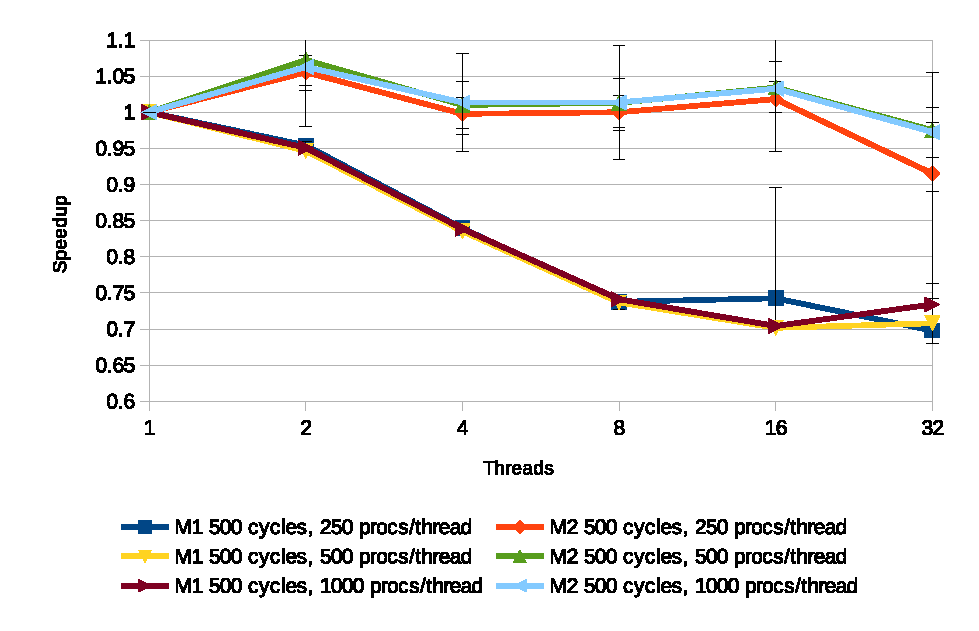
\includegraphics[width=\textwidth]{graphs/weak}
\caption[Weak scaling benchmark]{Weak scaling}
\label{fig:weak}
\end{figure}

\subsection{Discussion}
We can see that the continuous overhead of the atomic variable used in
the worker queue model is still clearly visible and appears to
increase with the level of parallelization. The statically
orchestrated model, on the other hand, produces much better results
and appear to show weak scaling properties with speedups within +/-
0.05. The performance of this model, however appears to drop when
going from 16 to 32 cores. This could be explained by the fact that we
performed the benchmarks on a on a 2x16 core machine This means, that
we cross CPU boundaries when going from 16 to 32 cores.

Contrary to our expectations, the work-per-cycle ratio is not clearly
visible in the results. The explanation for this may simply be that
the work-per-cycle ratios that we used in the benchmark weren't
sufficiently large. In the cycle dominated benchmark we used ratios of
10:1 and 1:10 respectively while in this benchmark we used ratios of
2:1, 1:1 and 1:2.


\section{Uneven workloads}
This benchmark, we attempt to confirm our conjecture that the work
list model will perform better than the statically orchestrated model
for networks coosisting of uneven workloads. This benchmark
essentially repeats the cycle dominated benchmark except that we
divide the processes on the ring evenly into two groups where one
group performs exactly one fourth as much work as the other. This
means, that we use the same process code as \cref{lst:cyclecode}
except that half of the processes will only run for 2500 iterations
instead of 10000 It's important to note that the processes in each of
these groups are laid out sequentially on the ring. since this will force the
statically orchestrated model into its worsts-case distribution of
workload.

The statically orchestrated model will thus spend a lot of time in the
synchronization barrier while the work list model will be able to
distribute load of the network much more evenly across the
threads. This benchmark is indeed very artificial, but it serves the
purpose of showing the strengths of the work list model

\begin{figure}
\centering
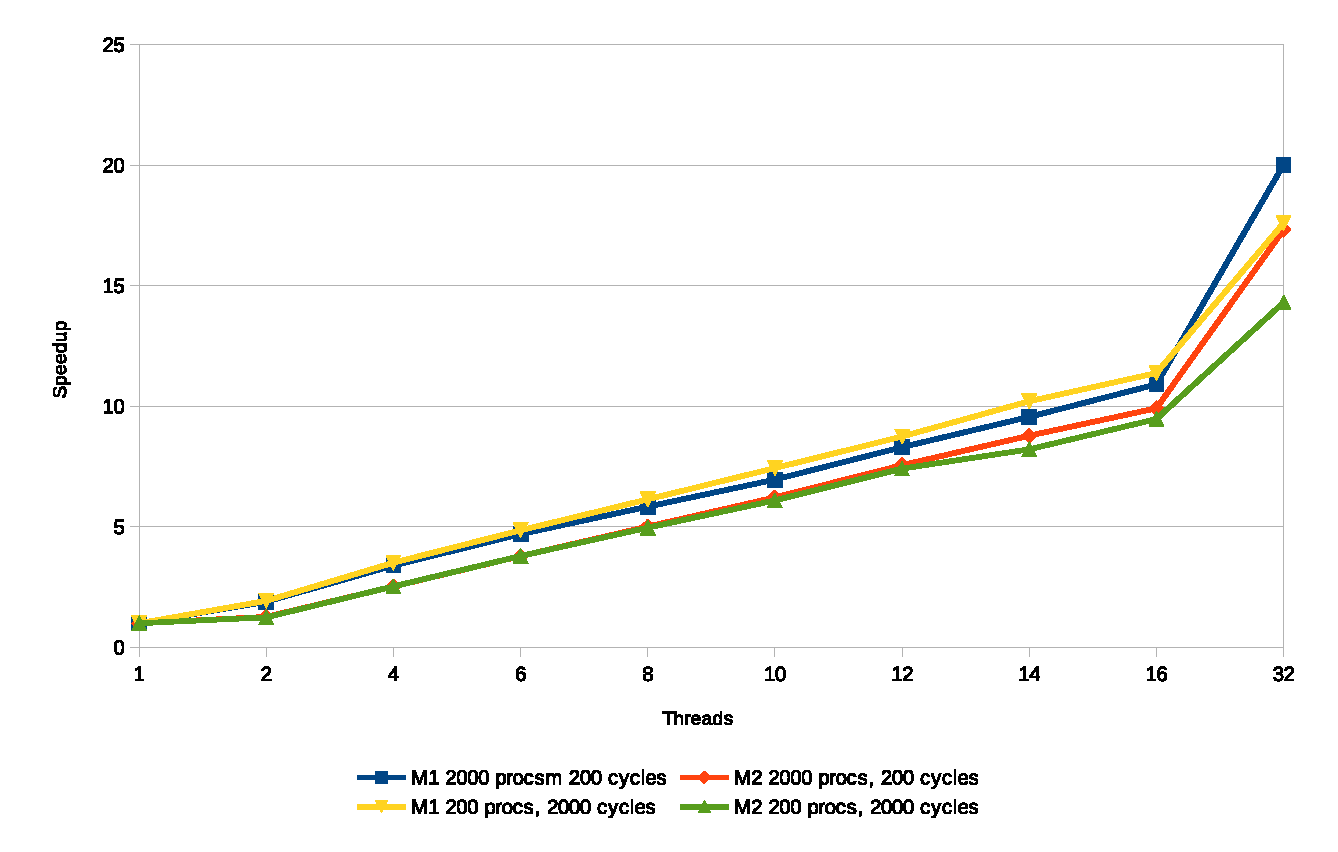
\includegraphics[width=\textwidth]{graphs/uneven}
\caption[Benchmark of uneven workloads]{The performance of the two
  parallelization models when executed on a network consisting of
  processes with a significant workload imbalance}
\label{fig:uneven}
\end{figure}

\subsection{Discussion}
This is the first benchmark where the work list model performed better
than the statically orchestrated model so the fundamental conclusion
is that our conjecture was confirmed. However, the difference between
the two models aren't as significant as we expected. It remains to be
seen whether the work list model would increase its advantage over the
statically orchestrated model if we increased the workload imbalances
between the processes even more but presumably, this would be the
case.

So, once again, the continuous synchronization of the work list model
proves disproportionately expensive.

\section{Future works}

BQueue with work stealing would be nice to implement, but as shown by
relevant benchmark using ``advanved'' datastructures for the process
queue comes at a significant cost. A way to implement work stealing
without increasing the cost of getting a process from the queue is
needed. Linearly pulling processes of a queue has a significant cache
advantage. Using work stealing to pull from ``the reverse'' would
reduce that advantage. 

All benchmarks has been largely artificial since they have been
targeted at exposing the advantages and disadvnatages of the
properties of the execution models that we have proposed  We need more real-world
samples to know where to actually tune the performance of system

More benchmarks:


The results that we have shown, although reasonable, can not be easily
explained by

\subsection{One-shot process orchestration}
In this model, we orchestrate the processes in our network as soon as
possible after execution start and

\subsection{Monte Carlo orchestration}
In this approach, we simply randomize the order of the processes. The
main advantage of this approach is that is computationally cheap
compared to

\subsection{Optimization-based orchestration}
Another way to orchestrate the processes is to use a


\subsection{Adaptive process orchestration}
The benefits of using a oneshot orchestration approach diminishes when
we execute process networks where the processes performs a variable
amount of work per iteration. In these kinds of networks, CPU-core
load distribution will gradually become uneven and suboptimal as the
network execution progresses. In order to keep this from happening and
maximize CPU-core utilization, we need to monitor process execution
time and core idle time as the network execution progresses. This is
what we refer to s adaptive orchestration. This approach, however
introduces another trade-off that we need to consider. producing an

\subsection{Adaptive Monte Carlo process orchestration}

\subsection{Adaptive Optimization-based process orchestration}



%%% Local Variables:
%%% mode: latex
%%% TeX-master: "master"
%%% TeX-command-extra-options: "-enable-write18"
%%% End:

\chapter{Conculsions}
% We have revealed some of the properties of SME. More real-world usage is still needed in order to decide on the optimal way to implement the network. We have given some options and shown that it is possible to support multiple execution models in the same framework. 

%%% Local Variables:
%%% mode: latex
%%% TeX-master: "master"
%%% TeX-command-extra-options: "-enable-write18"
%%% End:


\printbibliography

\appendix
\chapter{Benchmark data}
\label{chap:benchdata}
The tables below contain the raw results from our benchmarks.



%%% Local Variables:
%%% mode: latex
%%% TeX-master: "master"
%%% TeX-command-extra-options: "-enable-write18"
%%% End:



\end{document}

%%% Local Variables:
%%% mode: latex
%%% TeX-master: t
%%% TeX-command-extra-options: "-enable-write18"
%%% End:
